% S^0 (two points) with D^1 the segment between them, and D^2 a filled disk with
% boundary S^1. Source: book/tex/topology/constructions.tex (§ Spheres).
\documentclass[border=2mm]{standalone}
\usepackage{tikz}
\begin{document}
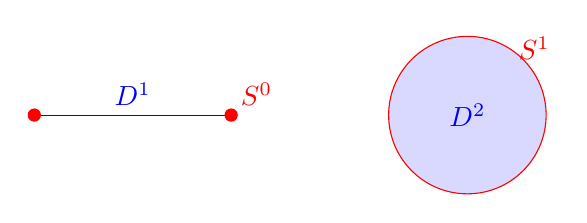
\begin{tikzpicture}[scale=1]
  % D^1 = segment, S^0 = its two endpoints
  \draw[blue] (-4,0) -- (-1.5,0) node[midway,above,blue] {$D^1$};
  \fill[red] (-4,0) circle (2.4pt);
  \fill[red] (-1.5,0) circle (2.4pt) node[above right,red] {$S^0$};
  % D^2 = filled disk, boundary S^1
  \fill[blue!15] (1.5,0) circle (1);
  \draw[red] (1.5,0) circle (1);
  \node[blue] at (1.5,0) {$D^2$};
  \node[red] at (2.35,0.85) {$S^1$};
\end{tikzpicture}
\end{document}
